
\begin{figure*}[tb]
    \centering
    \begin{subfigure}[b]{0.25\textwidth}
        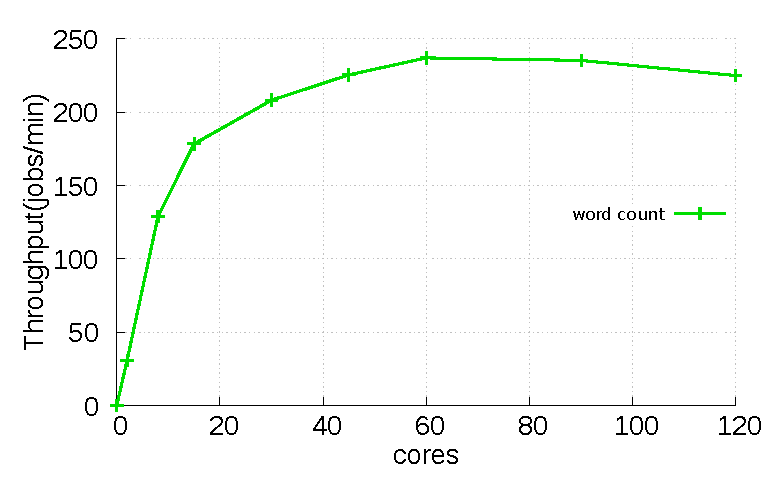
\includegraphics[width=1.8in]{graph/wc.eps}
        \caption{Word Count}
    \end{subfigure}%
    \begin{subfigure}[b]{0.25\textwidth}
        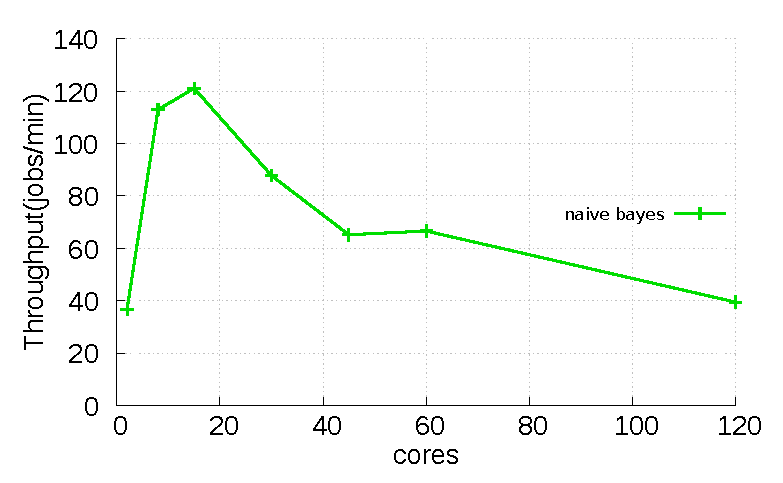
\includegraphics[width=1.8in]{graph/nb.eps}
        \caption{Naive Basian}
    \end{subfigure}%
    \begin{subfigure}[b]{0.25\textwidth}
        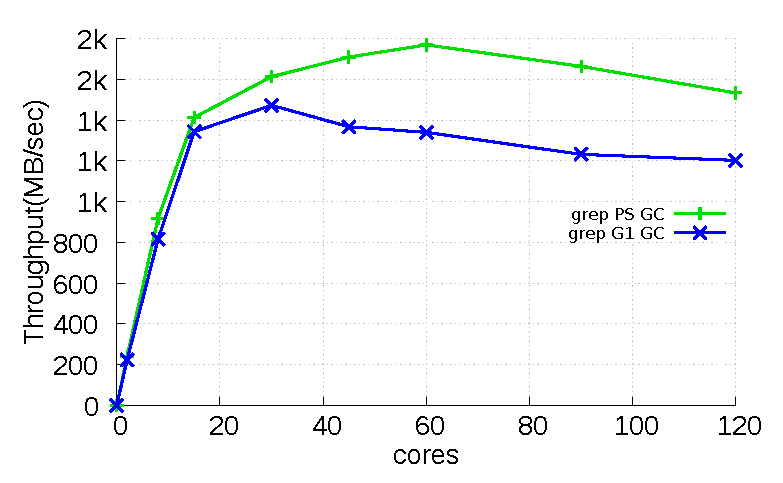
\includegraphics[width=1.8in]{graph/grep.eps}
        \caption{Grep}
    \end{subfigure}%
    \begin{subfigure}[b]{0.25\textwidth}
        \includegraphics[width=1.8in]{graph/kmeans.eps}
        \caption{K-means}
    \end{subfigure}%
    \caption{CPU utilization on 120 core.}
    \label{fig:utilization}
\end{figure*}



\begin{figure*}[tb]
    \centering
    \begin{subfigure}[b]{0.25\textwidth}
        \includegraphics[width=1.8in]{graph/wc_cpuutils.eps}
        \caption{Word Count}
    \end{subfigure}%
    \begin{subfigure}[b]{0.25\textwidth}
        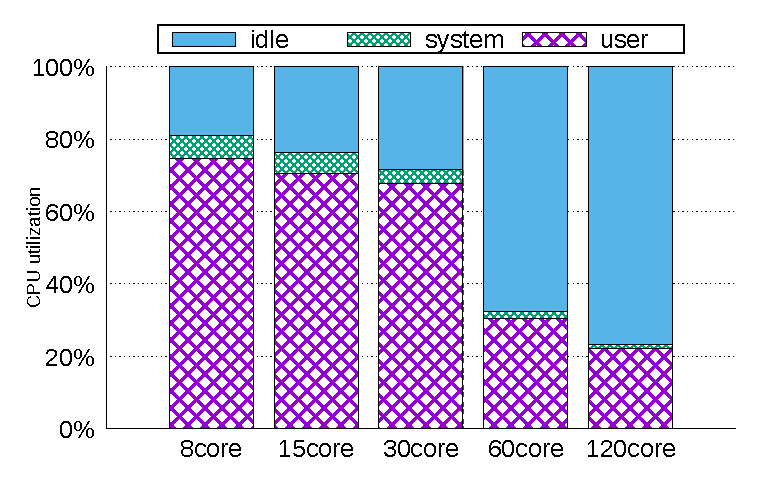
\includegraphics[width=1.8in]{graph/nb_cpuutils.eps}
        \caption{Naive Basian}
    \end{subfigure}%
    \begin{subfigure}[b]{0.25\textwidth}
        \includegraphics[width=1.8in]{graph/grep_cpuutils.eps}
        \caption{Grep}
    \end{subfigure}%
    \begin{subfigure}[b]{0.25\textwidth}
        \includegraphics[width=1.8in]{graph/kmeans_cpuutils.eps}
        \caption{K-means}
    \end{subfigure}%
        \centering
    \caption{CPU utilization on 120 core.}
    \label{fig:cpuutilization}
\end{figure*}

\section{Scale-up Server Scalalbility}




%$$$$$$$$$$$$$$$$$$$$$$$$$$$$$$$$$$$$$$$$$$$$$$$$$$$$$$$$$$$$$$$$$$$$$$$$$$$$$$$$
%$$$$$$$$$$$$$$$$$$$$$$$$$$$$$$$$$$$$$$$$$$$$$$$$$$$$$$$$$$$$$$$$$$$$$$$$$$$$$$$$
% 이번 장에 대한 설명
%$$$$$$$$$$$$$$$$$$$$$$$$$$$$$$$$$$$$$$$$$$$$$$$$$$$$$$$$$$$$$$$$$$$$$$$$$$$$$$$$
\ifkor
\else

\fi



\subsection{Test-bed and Benchmark}

%$$$$$$$$$$$$$$$$$$$$$$$$$$$$$$$$$$$$$$$$$$$$$$$$$$$$$$$$$$$$$$$$$$$$$$$$$$$$$$$$
%$$$$$$$$$$$$$$$$$$$$$$$$$$$$$$$$$$$$$$$$$$$$$$$$$$$$$$$$$$$$$$$$$$$$$$$$$$$$$$$$
% Apache Spark에 대한 설명
%$$$$$$$$$$$$$$$$$$$$$$$$$$$$$$$$$$$$$$$$$$$$$$$$$$$$$$$$$$$$$$$$$$$$$$$$$$$$$$$$
\ifkor
\noindent
\textbf{Apache Spark. }
Apache Spark is a framework for large scale distributed computation.
RDD(Resilient Distributed Datasets) is a collection of partitions of records, 
and the RDD is managed as LRU(Least Recently Used), so when there is not enough
memory, Spark evits the least recently used RDD.
Spark may has a substantial performance when dataset can fit in memory.

%\begin{figure}[h]
%    \centering
%    \begin{subfigure}[b]{0.22\textwidth}
%        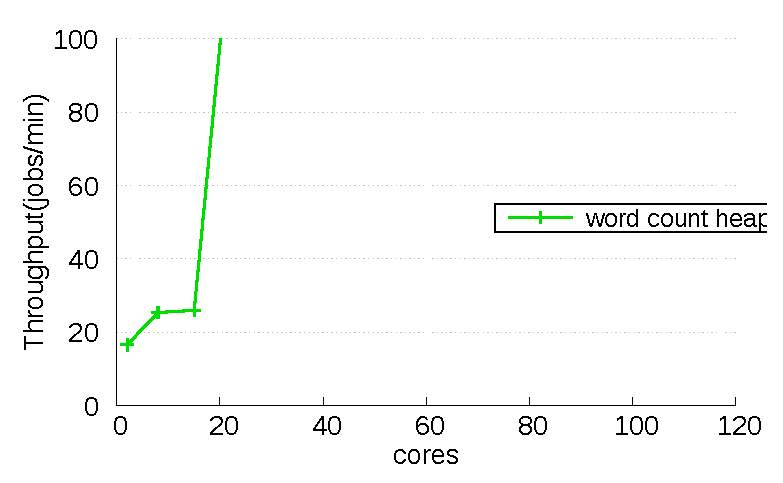
\includegraphics[width=1.5in]{graph/wc_max.eps}
%        \caption{Word Count}
%    \end{subfigure}%
%    \begin{subfigure}[b]{0.22\textwidth}
%        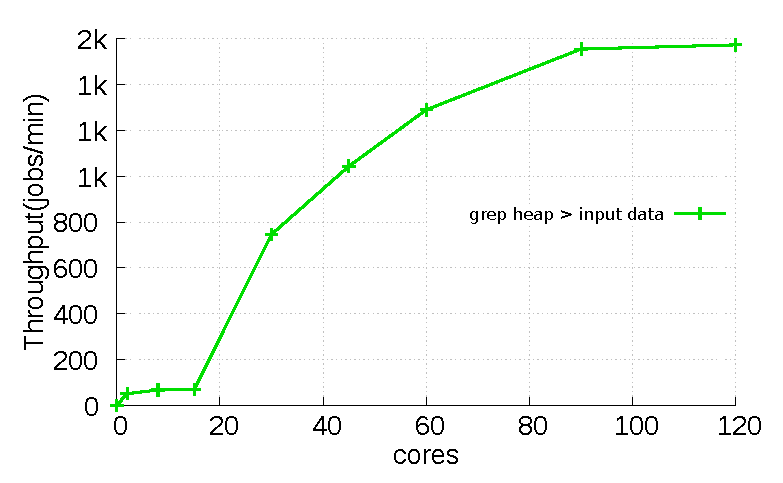
\includegraphics[width=1.5in]{graph/grep_max.eps}
%        \caption{Grep}
%    \end{subfigure}
%    \caption{CPU utilization on 120 core.}
%    \label{fig:utilization}
%\end{figure}

%Figure shows a substantial performance scalability of Spark when dataset can
% fit in memory(heap size > data size).
%However, large scale data(head size < data size) does not scale on scale-up
%server due to the GC and the memory latency.
\else
\fi

%$$$$$$$$$$$$$$$$$$$$$$$$$$$$$$$$$$$$$$$$$$$$$$$$$$$$$$$$$$$$$$$$$$$$$$$$$$$$$$$$
%$$$$$$$$$$$$$$$$$$$$$$$$$$$$$$$$$$$$$$$$$$$$$$$$$$$$$$$$$$$$$$$$$$$$$$$$$$$$$$$$
% 테스트 베드 설명
%$$$$$$$$$$$$$$$$$$$$$$$$$$$$$$$$$$$$$$$$$$$$$$$$$$$$$$$$$$$$$$$$$$$$$$$$$$$$$$$$
\ifkor
\noindent
\textbf{Test-bed. }
Our Intel platform is composed of Xeon E5 Each CPU exploits the Iby Brige
technoloy and consists in a multi-core architecture.
We use a machine to evaluate on real hardware: an 120-core (8 sockets × 15
cores) Intel Xeon E7-8870 (the same machine used for evaluation in chapter 9)
and, to show that our conclusions generalize.

\begin{figure}[h]
  \begin{center}
     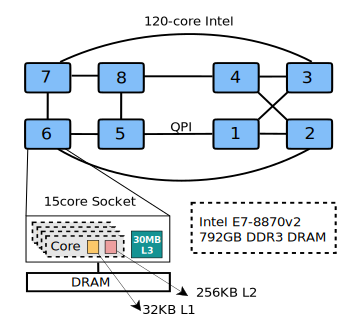
\includegraphics[width=0.4\textwidth]{fig/xeon}
  \end{center}
  \caption{test-bed intel xeon archtecture.}
  \label{fig:basic}
\end{figure}
Hyper-Threading is disabled, and Linux kernel 4.5-rc6.
\else

\fi

%$$$$$$$$$$$$$$$$$$$$$$$$$$$$$$$$$$$$$$$$$$$$$$$$$$$$$$$$$$$$$$$$$$$$$$$$$$$$$$$$
%$$$$$$$$$$$$$$$$$$$$$$$$$$$$$$$$$$$$$$$$$$$$$$$$$$$$$$$$$$$$$$$$$$$$$$$$$$$$$$$$
%Benchamrk에 대한 설명
%$$$$$$$$$$$$$$$$$$$$$$$$$$$$$$$$$$$$$$$$$$$$$$$$$$$$$$$$$$$$$$$$$$$$$$$$$$$$$$$$
\ifkor
\noindent
\textbf{Benchmark.} 벤치마크와 워크로드에 대한 BigData Benchmark를 사용하였다.
\begin{itemize}
\item \textbf{Word Count. }We have developed a novel lightweight log-based
structures with efficient log management implementation.
\item \textbf{Grep. }
We applied the in Linux kernel to two reverse mapping(anonymous, file) on
Our design improved throughput and execution time from 1.5x through 2.7x on 120 core.
\item \textbf{Naive Basian. }
We applied the in Linux kernel to two reverse mapping(anonymous, file) on
Our design improved throughput and execution time from 1.5x through 2.7x on 120 core.
\item \textbf{K-means.}
We applied the in Linux kernel to two reverse mapping(anonymous, file) on
Our design improved throughput and execution time from 1.5x through 2.7x on 120 core.
\end{itemize}
\else

\fi


\subsection{Spark Scalability Problem}
%$$$$$$$$$$$$$$$$$$$$$$$$$$$$$$$$$$$$$$$$$$$$$$$$$$$$$$$$$$$$$$$$$$$$$$$$$$$$$$$$
%$$$$$$$$$$$$$$$$$$$$$$$$$$$$$$$$$$$$$$$$$$$$$$$$$$$$$$$$$$$$$$$$$$$$$$$$$$$$$$$$
%Scalability 결과에 대한 대략 적인 설명
%$$$$$$$$$$$$$$$$$$$$$$$$$$$$$$$$$$$$$$$$$$$$$$$$$$$$$$$$$$$$$$$$$$$$$$$$$$$$$$$$
\ifkor
Figure 1 shows the spark scalability of five workloads with G1 and Parallel
Scavenge GC(PS).
Up to 60 core, The five workloads scales linealy and then GC pause become
bottlenecks.
The word count flattens out after 60 core, but other benchmarks slightly go
down because not only GC overhead but also NUMA effects. 
To evalute state of the art GC, we used G1 and PS GC.
The result of impact of chainging the GC are PS GC results in 3.3x better
performance than G1 GC on 120 core.
However, although we used the scalable GC, the Spark performance scalabiliy is
still limited by GC and NUMA effects.
\else

\fi


%$$$$$$$$$$$$$$$$$$$$$$$$$$$$$$$$$$$$$$$$$$$$$$$$$$$$$$$$$$$$$$$$$$$$$$$$$$$$$$$$
%$$$$$$$$$$$$$$$$$$$$$$$$$$$$$$$$$$$$$$$$$$$$$$$$$$$$$$$$$$$$$$$$$$$$$$$$$$$$$$$$
%CPU utilization에 대한 설명
%$$$$$$$$$$$$$$$$$$$$$$$$$$$$$$$$$$$$$$$$$$$$$$$$$$$$$$$$$$$$$$$$$$$$$$$$$$$$$$$$

\ifkor
Figure ~\ref{fig:cpuutilization} shows the job's CPU utilization.
Our goal is high cpu utilization, 
Th y-axis is the percentage of time spent in kernel-space code(sys), user-space
code(user), and idle time(idle).
When core counts increase, all benchmarks increase idle time due to GC pasue
that means 

\else

\fi


%$$$$$$$$$$$$$$$$$$$$$$$$$$$$$$$$$$$$$$$$$$$$$$$$$$$$$$$$$$$$$$$$$$$$$$$$$$$$$$$$
%$$$$$$$$$$$$$$$$$$$$$$$$$$$$$$$$$$$$$$$$$$$$$$$$$$$$$$$$$$$$$$$$$$$$$$$$$$$$$$$$
% Linux kernel scalability (lock, cache cohearnci, scheduler)등등 OS 노이즈에 대한 설명
%$$$$$$$$$$$$$$$$$$$$$$$$$$$$$$$$$$$$$$$$$$$$$$$$$$$$$$$$$$$$$$$$$$$$$$$$$$$$$$$$
\ifkor
%NUMA의 영향 뿐만 아니라, 추가적으로 operating system의 scalability 저해 요소 때문에 
%파티션닝 방법은 필요하다.
%우리는 operation system에서 scalability의 영향을 주는 것을 확인하기 위해 가장먼저
%lock을 조사해보았다.
%첫째로 공유 데이터를 lock이 있다. 표 xxx 앞에서 실험한 spark의 wordcount에 대해서 .
%JVM 위에서 동작하는 thread간의 공유하는 single address space때문에 발생하는 공유 문제이다.
%다음으로 scheduler가 아직 
%마지막으로 cache cohearci traffic이 있다. 
\else

\fi



\subsection{Benefit of JVM Partitioning}
%\subsection{NUMA}

%$$$$$$$$$$$$$$$$$$$$$$$$$$$$$$$$$$$$$$$$$$$$$$$$$$$$$$$$$$$$$$$$$$$$$$$$$$$$$$$$
%$$$$$$$$$$$$$$$$$$$$$$$$$$$$$$$$$$$$$$$$$$$$$$$$$$$$$$$$$$$$$$$$$$$$$$$$$$$$$$$$
%NUMA 영향에 대한 대략 적인 설명
%$$$$$$$$$$$$$$$$$$$$$$$$$$$$$$$$$$$$$$$$$$$$$$$$$$$$$$$$$$$$$$$$$$$$$$$$$$$$$$$$

\ifkor
Spark and Hadoop ramework use JAVA and it needs java virtual machine, so
understanding the partitioning effect on JVM is importance.
To preliminarily analysis the JVM partitioning effect, we conducted
benchamrk using SPECjbb2013, which a state of the art benchmark for
JVM performance.
We used two different experiment settings. First, we used per-socket
JVM partitioning using the numa control application(numactl).
Second, we set maxium available memory to JVM heap size and
threads are scheduled by the OS in order to migrate any core, and we
enable automatic NUMA balancing feature in the Linux kernel.
\else
\fi

\begin{figure}[h]
  \begin{center}
     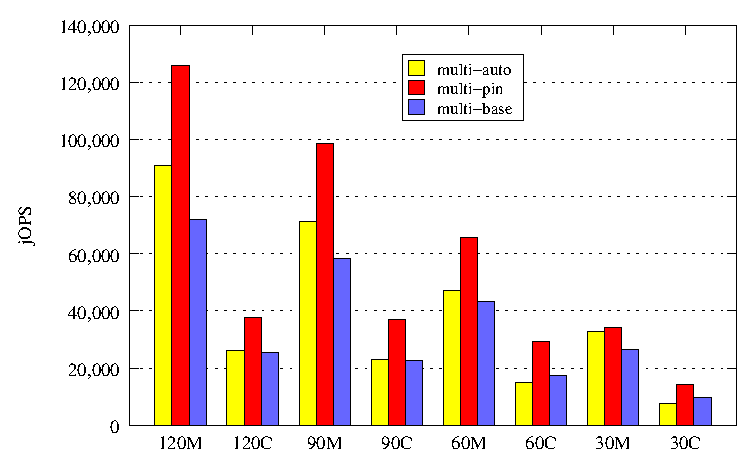
\includegraphics[width=0.4\textwidth]{graph/SPECjbb2013}
  \end{center}
  \caption{Test-bed Intel xeon archtecture.}
  \label{fig:basic}
\end{figure}

\ifkor

The results all core shows that partitioning approach outperforms than
non-partitioning approach by Xx on 120 core.
In manycore scale-up server, partiting approach has best performance
scalability.
\else
\fi
